\chapter{Arbeitspakete}
Die einzelnen Arbeitspakete werden Mithilfe vom Projektverwaltungstools Redmine organisiert. Für die Betreuer wurde ein eigener Zugang zum Redmine-Projekt eingerichtet.

\section{Gastzugang Redmine}
http://152.96.192.44/redmine \\
Zugang: guest / zurich2Rapperswil \\

\begin{landscape}
\section{Arbeitspakete}
	% Pdf erst erneuern, wenn Projektplan fertig
	\begin{figure}[H]
		\centering
			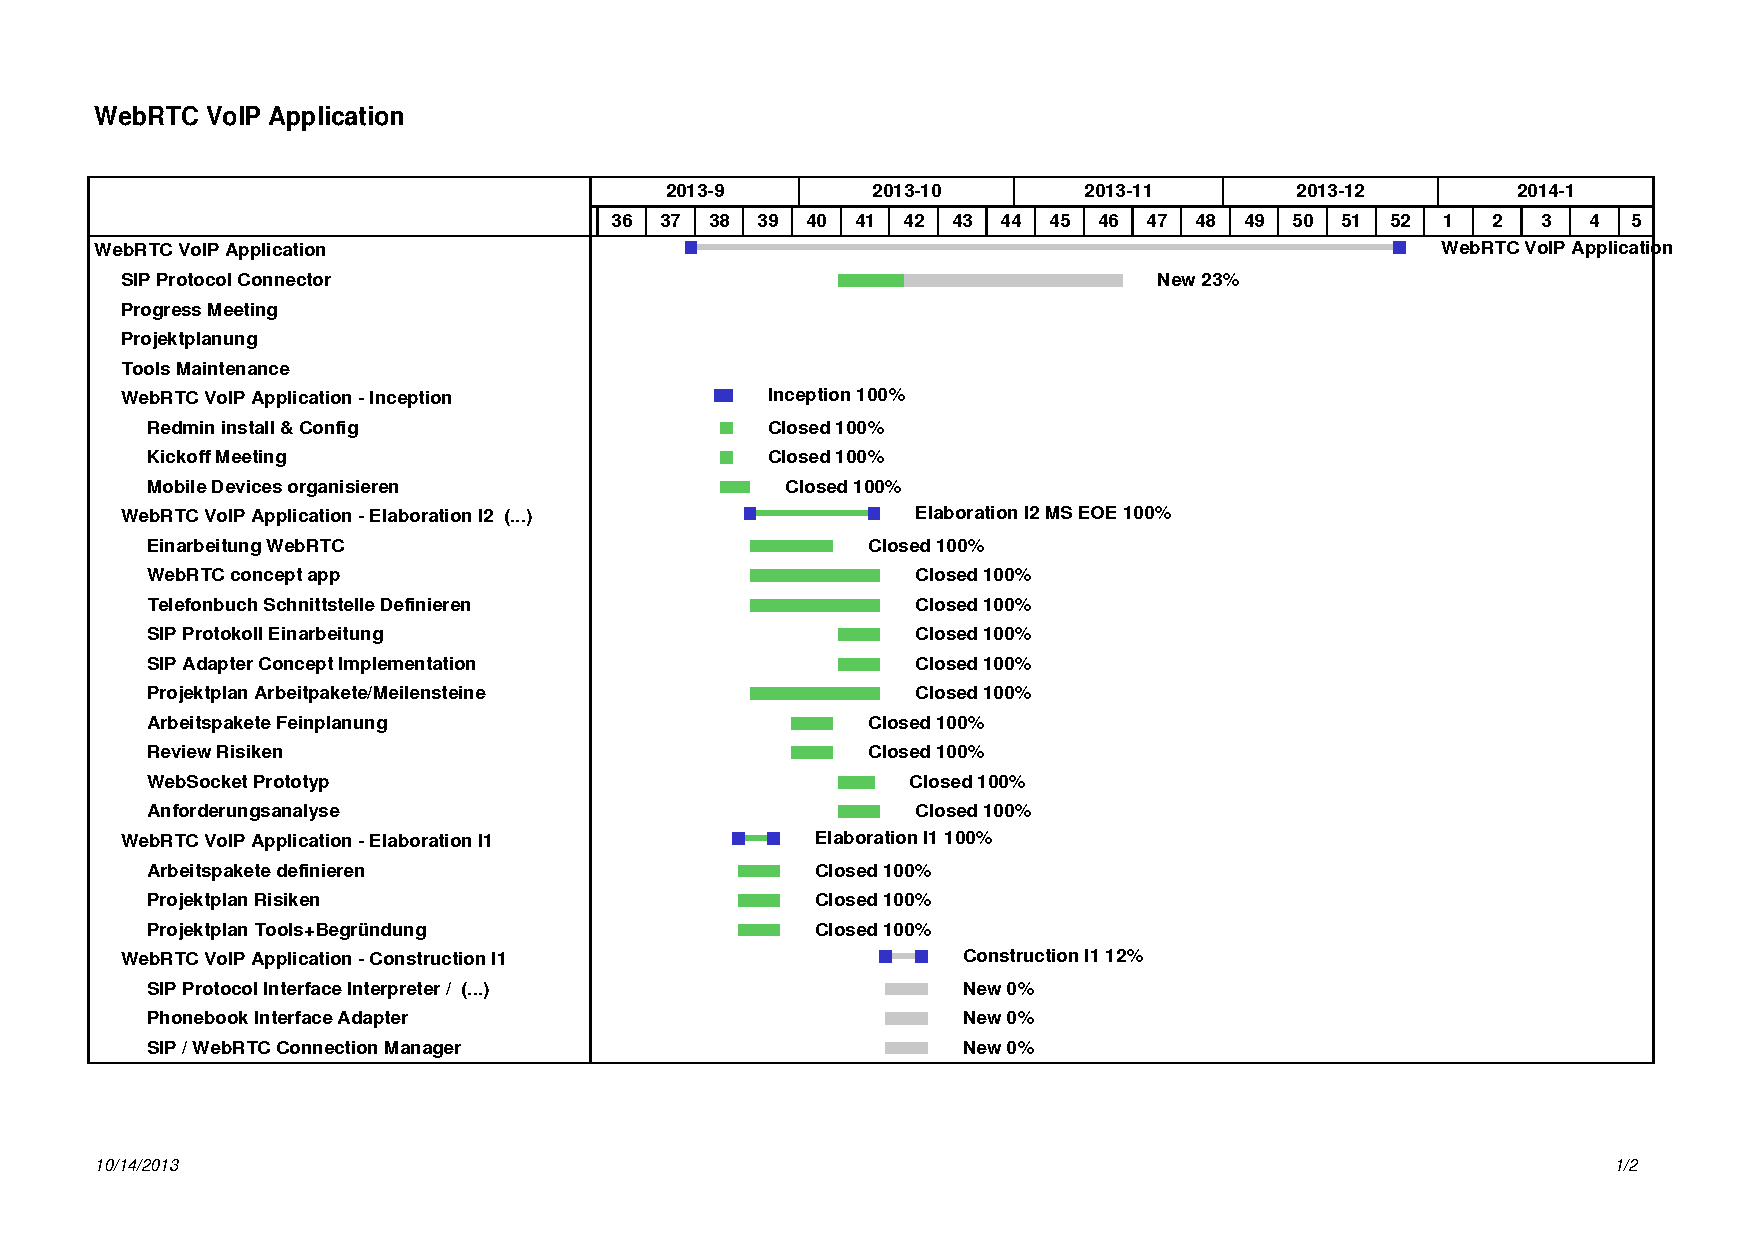
\includegraphics[trim=1.5cm 2.5cm 1cm 3cm, clip=true,page=1,width=1.4\textwidth]{media/jsvoipcommunication-gantt.pdf}
			\caption[ArbeitpaketeUndMeilstones]{Arbeitspakete und Milestones}
			\label{flowDiagramm1}
	\end{figure}
	\begin{figure}[H]
		\centering
			\includegraphics[trim=1.5cm 10cm 1cm 0cm, clip=true,page=2,width=1.4\textwidth]{media/jsvoipcommunication-gantt.pdf}
			\caption[ArbeitpaketeUndMeilstones]{Arbeitspakete und Milestones}
			\label{flowDiagramm1}
	\end{figure}

\end{landscape}